\documentclass[12pt]{amsart}
\usepackage{amsmath,amssymb,url,color,tikz}
\usetikzlibrary{patterns} 
\usepackage[all]{xy}
\usepackage{young}
\usepackage{enumerate}
\usepackage[margin=1in]{geometry}
\usepackage{hyperref}
\usepackage{graphicx}
\usepackage{caption} 
\usepackage{subcaption}
\usetikzlibrary{arrows,automata}
\usepackage[colorinlistoftodos,color=red!70]{todonotes}

%\oddsidemargin = 0.0cm \evensidemargin = 0.0cm \textwidth = 6.5in
%\textheight =8.5in


\newtheorem{thm}{Theorem}
\newtheorem{lem}[thm]{Lemma}
\newtheorem{prop}[thm]{Proposition}
\newtheorem{cor}[thm]{Corollary}
\newtheorem{conj}[thm]{Conjecture}
\newtheorem{qn}[thm]{Question}

\theoremstyle{definition}
\newtheorem{defn}[thm]{Definition}
\newtheorem{ex}[thm]{Example}

\theoremstyle{remark}
\newtheorem{rem}[thm]{Remark}

\numberwithin{thm}{section}

\newcommand{\RR}{\mathbb{R}}
\newcommand{\ZZ}{\mathbb{Z}}
\newcommand{\mcO}{\mathcal{O}}

\newcommand{\minho}[1]{\todo[color=yellow,inline]{minho: #1}}
\newcommand{\doyeob}[1]{\todo[color=blue!70,inline]{doyeob: #1}}
\newcommand{\mario}[1]{\todo[color=red,inline]{mario: #1}}
\newcommand{\emily}[1]{\todo[color=gray,inline]{emily: #1}}
\newcommand{\chensu}[1]{\todo[color=orange,inline]{chensu: #1}}
\newcommand{\morgan}[1]{\todo[color=green,inline]{morgan: #1}}
\newcommand{\chaiwah}[1]{\todo[color=pink,inline]{chaiwah: #1}}

\renewcommand{\qedsymbol}{$\blacksquare$}
\def\<{\langle}
\def\>{\rangle}
\def\longto{\longrightarrow}

\begin{document}


\title{Team 4 (Fast and Somewhat Accurate Algorithms): Mathematical Modeling in Industry XIX (August 5-14, 2015)}
\author[Wu]{Chai Wah Wu, IBM (mentor)}
\author[Barela]{Mario Barela}
%, The University of Iowa}
\author[Chen]{Su Chen}
%, University of Kansas}
\author[Gunawan]{Emily Gunawan}
%, University of Minnesota}
\author[Schreffler]{Morgan Schreffler}
%, University of Kentucky}
\author[Song]{Minho Song}
%, Sungkyunkwan University
\author[Yeo]{Doyeob Yeo}
%, Korea Advanced Institute of Science and Technology (KAIST)}


\date{\today}
\maketitle

%%=======================================
\section{Introduction}
%%=======================================
We seek to produce algorithms using look-up-tables (LUT) for speeding up edge-detection and blurring filters. In order for any LUT-based algorithm to be useful, the size of the LUTs need to be reasonably small. To meet this aim, we use:
\begin{enumerate}
\item a byte-truncation technique, 
\item convolution decompositon of a kernel $3\times 3$ matrices (rank one),
\item approximate convolution decompositon of a kernel $3\times 3$ matrices (rank two)
\item and taking advantage of the observation that edge-detection algorithm shows higher tolerance to byte-truncation. 
\end{enumerate}

%%=================================
\section{instruction for using comments (while we are drafting the report)}

\morgan{to write a comment to Morgan}
\mario{to write a comment to Mario}
\minho{to write a comment}
\chensu{to write a comment}
\emily{to write a comment}
\doyeob{to write a comment}
\chaiwah{to write a comment}

\section{Wednesday August 5: Daily Notes}
Decide that look-up tables  are not suitable for a median filter algorithm.

\section{Thursday August 6: Daily Notes}
\subsection{Compute an algorithm using a look-up table for a high-pass kernel matrix} 
$\frac{1}{8}
\begin{bmatrix}
0 & -1 & 0\\
-1 & 4 & -1\\
0 & -1 & 0
\end{bmatrix}$ using a truncation technique using truncation matrix
$\begin{bmatrix}
8 &4 &8\\
4 &2 &4\\
8 &4 &8
\end{bmatrix}$. This particular look-up table was created in about 15-19 seconds.

\subsection{
Compare results of linear filters on Matlab with and without truncating digits}
Truncating with the following truncating matrices look acceptable for gray-scale images:
$
T_0=
\begin{bmatrix}
0 &4 &0\\
4 &0 &4\\
0 &4 &0
\end{bmatrix},
T_1=
\begin{bmatrix}
0 &4 &0\\
4 &1 &4\\
0 &4 &0
\end{bmatrix}
T_2=
\begin{bmatrix}
0 &4 &0\\
4 &2 &4\\
0 &4 &0
\end{bmatrix}
T_3=
\begin{bmatrix}
0 &5 &0\\
5 &3 &5\\ 
0 &5 &0
\end{bmatrix}
T_4=
\begin{bmatrix}
0 &3 &0\\
3 &1 &3\\
0 &3 &0
\end{bmatrix}
.$

A normalized gradient magnitude from Sobel-Feldman operator \cite{Wikipedia/Sobel}
$\mathbf{G} = \sqrt{ {\mathbf{G}_x}^2 + {\mathbf{G}_y}^2 }$

where

$\mathbf{G}_x = \begin{bmatrix} 
 -1 & 0 & +1  \\
-2 & 0 & +2 \\
-1 & 0 & +1 
\end{bmatrix} * \mathbf{A}
\quad
\mbox{and}
\quad   
\mathbf{G}_y = \begin{bmatrix} 
-1 & -2 & -1 \\
 0 & 0 & 0 \\
+1 & +2 & +1
\end{bmatrix} * \mathbf{A}$.

Here * denotes the 2-dimensional convolution operation.

Some high-pass kernel matrices:
\begin{itemize}
\item
$
\frac{1}{8}
\begin{bmatrix}
0 & -1 & 0\\
-1 & 4 & -1\\
0 & -1 & 0
\end{bmatrix}$
\item
$
\frac{1}{8}
\begin{bmatrix}
-1 & -1 & -1\\
-1 & 8 & -1\\
-1 & -1 & -1
\end{bmatrix}$
\end{itemize}

A low-pass kernel matrix:
\begin{itemize}
\item
$
\frac{1}{16}
\begin{bmatrix}
1 & 2 & 1\\
2 & 4 & 2\\
1 & 2 & 1
\end{bmatrix}$
\end{itemize}

A Scharr Gradient kernel matrix:
\begin{itemize}
\item
$
\frac{1}{32}
\begin{bmatrix}
3 & 10 & 3\\
0 & 0 & 0\\
-3 & -10 & -3
\end{bmatrix}$
\end{itemize}

An unsharp mask kernel filter:
\begin{itemize}
\item
$
\frac{1}{8}
\begin{bmatrix}
0 &-\lambda &0\\
-\lambda &1-0.3*\lambda &-\lambda\\
0 &-\lambda &0
\end{bmatrix}
$
where $\lambda=0.1$.
\end{itemize}
%%=================================

\rem{For blurring filters (including the low-pass kernel we list above), we think that the truncation technique will cause too many errors.}


\subsection{Matrix-decomposition?}
Started looking into doing matrix decomposition to make the LUT smaller.

\subsection{Using the truncating technique for a blurring filter: Taking advantage of the fact that truncating works better for edge-detecting than for blurring}

\begin{rem}\label{rem:sharpening_vs_blurring}
\begin{enumerate}
\item The truncation method $T$ can be used to reduce running time.
\item Truncation introduces too much error for blurring, but is decent for edge-detecting.
\end{enumerate}
\end{rem}

Let $I$, $L$, and $H$ denote the identity, a low-pass filter operation, and a high-pass filter operation on an image.
Let $L(T)$, and $H(T)$ denote $L$ and $H$ with a truncation using the truncation matrix $T$.
To informally say that applying a truncation technique to a high-pass filter gives close enough result, we can write $H \approx H(T)$.

Since $I = L + H$, we have
$L = I - H \approx I - H(T)$.

\begin{ex}
For example, consider a high-pass filter
$H=
\frac{1}{8}
\begin{bmatrix}
0 & -1 & 0\\
-1 & 4 & -1\\
0 & -1 & 0
\end{bmatrix}$.
Let $$
T_{1}=\left[
\begin{array}{ccc}
8 & 4 & 8 \\
4 & 2 & 4 \\
8 & 4 & 8
\end{array}
\right] ,T_{2}=\left[
\begin{array}{ccc}
8 & 5 & 8 \\
5 & 3 & 5 \\
8 & 5 & 8
\end{array}
\right] \mbox{ and }T_{3}=\left[
\begin{array}{ccc}
8 & 6 & 8 \\
6 & 4 & 6 \\
8 & 6 & 8
\end{array}
\right]
$$
be truncation matrices. The table\ref{table:comparison_of_errors} shows us how $L(T_i)$ and $I-H(T_i)$ are different from the low-pass filter $L=I-H$ for each $i$. $L(T_i)$ is Old and $I-H(T_i)$ is New in the table\ref{table:comparison_of_errors}.

\begin{table}[ht]
\begin{center}
\begin{tabular}{c|c|c|c|c|c|c|}
\cline{2-7}  & \multicolumn{2}{|c|}{$T_{1}$} &
\multicolumn{2}{c|}{$T_{2}$} & \multicolumn{2}{c|}{$T_{3}$}
\\\cline{2-7} & Old & New & Old & New & Old & New \\\hline \multicolumn{1}{ |c| }{PSNR} &
38.12 & 39.58 & 30.80 & 32.84 & 22.59 & 25.59 \\\hline
\multicolumn{1}{ |c| }{$l_{2}$ - error} &0.011 & 0.012 & 0.029 & 0.023 &
0.074 & 0.053 \\\hline \multicolumn{1}{ |c| }{$l_{\infty
}$ -
error} & 0.033 & 0.029 & 0.077 & 0.062 & 0.17 & 0.14 \\
\hline
\end{tabular}
\bigskip
\caption{Comparison of errors}
\label{table:comparison_of_errors}
\end{center}
\end{table}
\doyeob{Please add paper references for  PSNR}
$l_2$, $l_{\infty}$-differences between two images A,B are given as:
\begin{displaymath}
l_2\textrm{-difference} = \sqrt{ \frac{ \sum_{i,j} \left\{ A(i,j) - B(i,j) \right\}^2} {\textrm{(size of image)}}}
\end{displaymath}
\begin{displaymath}
l_{\infty}\textrm{-difference} = \textrm{max}_{i,j} \left \vert A(i,j) - B(i,j) \right\vert .
\end{displaymath}

The PSNR (in dB) is defined as
\begin{displaymath}
\begin{array}{ccl}
\textrm{PSNR} & = & 10\cdot \textrm{log}_{10} \left( \frac{\textrm{MAX}_B^2}{\textrm{MSE}} \right)\\
		 & = & 20 \cdot \textrm{log}_{10} \left( \frac{\textrm{MAX}_B}{\sqrt{\textrm{MSE}}} \right)
\end{array}
\end{displaymath}
where
\begin{displaymath}
\textrm{MSE} = \frac{1}{(\textrm{size of image})}  \sum_{i,j} \left\{ A(i,j) - B(i,j) \right\}^2.
\end{displaymath}
PSNR can be easily calculated by using MATLAB command $psnr(A,B)$.
PSNR is the abbreviation for Peak Signal-to-Noise Ratio. In brief, it shows us how image is different. As PSNR is higher, it becomes harder to recognize the difference between original image and filtered image. Typical values for the PSNR in lossy image are between 30 and 50 dB, provided the bit depth is 8 bits. 
As you see, our new approach gives us the better results no matter which truncation matrix you use.
See also Figures \ref{fig:comp} made via the truncation matrix $T_3$.
\begin{figure}[h] \centering 
\begin{subfigure}[b]{0.3\textwidth} 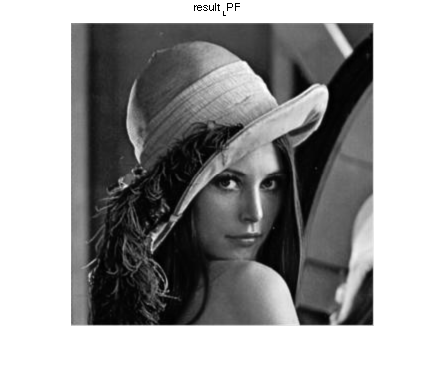
\includegraphics[width=\textwidth]{LPF.png} \caption{LPF} \label{fig:LPF} \end{subfigure}
\begin{subfigure}[b]{0.3\textwidth} 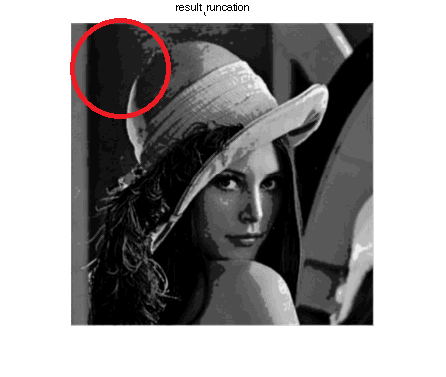
\includegraphics[width=\textwidth]{truncation.png} \caption{LPF with Truncation} \label{fig:LPF with Truncation} \end{subfigure}
\begin{subfigure}[b]{0.3\textwidth} 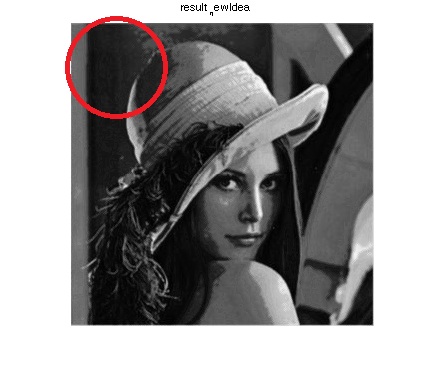
\includegraphics[width=\textwidth]{new.png} \caption{Result of the New Idea} \label{fig:new} \end{subfigure}
\caption{Comparison of filtered images}\label{fig:comp} 
\end{figure}

As you see, you can easily check that our new idea reduces staircase effects against the usual truncation method.
\end{ex}

Likewise, we can apply our method to any other low-pass filter as follows:

\begin{itemize}
\item[1.] Let $L$ be the our target low-pass filter.
\item[2.] Set $\tilde{H}:=I-L(T)$ for a certain truncation $T$.
\item[3.] Find $\tilde{L}:=I-\tilde{H}$ as an approximation of $L$.
\end{itemize}

Note that the second and third step stands for avoiding staircase effects.
\section{Friday August 7}

Group meeting
\begin{enumerate}
\item Testing filters with truncation
\item Generating LUT to match with above.
\item Decomposition into multiple LUTs.
\item $L \approx Id - H(T)$
\item Color (RGB) filters (see what Matlab does with edge detection for color pictures to make sure we are doing filters correctly.)
\item Sobel / Scharr magnitude operator (see what Matlab does with color).
\end{enumerate}

\subsection{A rank 1 decomposition}
Truncation can be a very powerful tool we can use to reduce the size of our LUTs. We of course have to be aware of the errors we sacrifice for computation time. In effort to reduce the size of our LUTs before truncation we explore a decomposition of our kernal K.
\\
\textbf{Idea:}
For any $(n\times n)$ matrix K that has rank 1 we can decompose the matrix $K$ as:
$$K=c*b^T$$
where $c,b \in \mathbb{R}^n$ and ``*" represents the matrix convolution. The convolution of two $n-dimensional$ vectors is actually the same a multiplication of the two vectors. 
\\
\textbf{Example:}
Consider the 
Low-pass filter K below and the decomposition.
$$
\begin{bmatrix}
1 & 2 & 1\\
2 & 4 & 2\\
1 & 2 & 1
\end{bmatrix}
=
\begin{bmatrix}
 1\\
 2\\
 1
\end{bmatrix}
\begin{bmatrix}
1 & 2 & 1\\
\end{bmatrix}
$$


Exploiting symmetry (or not necessarily).
$$
\begin{bmatrix}
1 & 2 & 1\\
2 & 4 & 2\\
1 & 2 & 1
\end{bmatrix}
=
\begin{bmatrix}
0 & 1 & 0\\
0 & 2 & 0\\
0 & 1 & 0
\end{bmatrix}
*
\begin{bmatrix}
0 & 0 & 0\\
1 & 2 & 1\\
0 & 0 & 0
\end{bmatrix}
$$
Optimization toolbox in Matlab:
$fminunc(f, x_o)$.

Try $||H_{\text{high-pass kernel}} - M*N||_{\text{FRO or something else}}$.

\mario{is writing the code.}

\subsection{More matrix decomposition}
Morgan had an idea to take advantage of this:
$$
\begin{bmatrix}
-1 & -1 & -1\\
-1 & 8 & -1\\
-1 & -1 & -1
\end{bmatrix}
=
\begin{bmatrix}
 1\\
 1\\
 1
\end{bmatrix}
\begin{bmatrix}
-1 & -1 & -1\\
\end{bmatrix}
+
\begin{bmatrix}
0 & 0 & 0\\
0 & 9 & 0\\
0 & 0 & 0
\end{bmatrix}
$$

\subsection{Sobel magnitude filter}
Ran an RGB picture with Mario's color code and the results look similar as the one in Wikipedia (but not as nice), and the results look acceptable even with truncating to 5,6 digits.

\section{Saturday}

\subsection{A rank 2 decomposition approximation}
Recall that a rank 1 decomposition of our kernal $K$ had the form $$
K=c*b^T
$$
where $c,b \in \mathbb{R}^n$. This resulted in two LUTs of size $2^{24}$ bytes instead of the full LUT of size $2^{72}$ bytes. This drastically reduces the size of the LUT before any truncation but it requires us to have a rank 1 kernal $K$. What can we do for a filter that is not rank 1?
\\
\textbf{Question: Can we decompose the filter $K$   in a better way?}
\\
Consider the decomposition of our $(3\times 3)$filter $K$ into the convolution:
$$K=A*B$$
where 


$$
A
=
\begin{bmatrix}
a & b & 0\\
c & d & 0\\
e & f & 0
\end{bmatrix}
,
B=
\begin{bmatrix}
g & h & i\\
k & m & n\\
0 & 0 & 0
\end{bmatrix}$$
\\
Ran an algorithm using fmin

$$
\begin{bmatrix}
-1 & -1 & -1\\
-1 & 8 & -1\\
-1 & -1 & -1
\end{bmatrix}
=
\begin{bmatrix}
a & d & 0\\
b & e & 0\\
c & f & 0
\end{bmatrix} *
\begin{bmatrix}
g & h & i\\
j & k & \ell \\
0 & 0 & 0
\end{bmatrix}
$$

$
A =
\begin{bmatrix}
  -0.372739294911747  &-0.443690961374357 & -0.457110102971229\\
  -0.509997537573061  & 2.683304035822869 &                  0\\
                   0  &                 0 &                  0
\end{bmatrix}
$

$
B =
\begin{bmatrix}
                   0&                   0&                   0\\
                   0&   2.681646089142412&  -0.509741093569434\\
  -0.456856367067759&  -0.443428387610633&  -0.372501463359094
\end{bmatrix}
$

\text{conv2(A,B,'same')}\\
$
\begin{bmatrix}
  -0.999554872469786  &-0.999821595552767  &-0.999640004082445\\
  -0.999646676848929  & 8.000063237563769  &-0.999819205287410\\
  -0.999737147772875  &-0.999878353018540  &-0.999534679981381
  \end{bmatrix}
$
  
  norm(F-conv2(A,B,'same'),'fro')

ans =

     $9.063656510413503e-04$

\section{ideas about what to do (Emily)}
\begin{itemize}

\item Filter color images with these 
http://r0k.us/graphics/kodak/

\end{itemize}

\section{Monday}
\emily{todo: Check errors $||L(A-B)||_{F}$ where $L$ is a low-pass filter. Our eyes are essentially a low-pass filter. Chai thinks that PSNR-HVS is essentially this.}

\begin{thebibliography}{widest entry}
\bibitem[Wikipedia/Sobel]{Wikipedia/Sobel} {Sobel operator}%{https://en.wikipedia.org/wiki/Sobel_operator}
\end{thebibliography}
\end{document}